%%%%%%%%%%%%%%%%%%%%%%%%%%%%%%%%%%%%%%%%%%%%%%%%%%%%%%%%%%%%%%%%
%
% Copyright (C) 2017-2019 Tactical Computing Laboratories, LLC
% All Rights Reserved
% contact@tactcomplabs.com
%
%%%%%%%%%%%%%%%%%%%%%%%%%%%%%%%%%%%%%%%%%%%%%%%%%%%%%%%%%%%%%%%%

%----------------------------------------------------------------------------------------
%	PACKAGES AND DOCUMENT CONFIGURATIONS
%----------------------------------------------------------------------------------------

\documentclass{article}

\usepackage[margin=1.0in]{geometry}
\usepackage[version=3]{mhchem} % Package for chemical equation typesetting
\usepackage{siunitx} % Provides the \SI{}{} and \si{} command for typesetting SI units
\usepackage{graphicx} % Required for the inclusion of images
%\usepackage{natbib} % Required to change bibliography style to APA
\usepackage{amsmath} % Required for some math elements 
\usepackage[utf8]{inputenc}
\usepackage[english]{babel}
\usepackage[parfill]{parskip}
\usepackage{array}
\usepackage{algorithm}
\usepackage{algcompatible}
\usepackage{listings}
\usepackage{xcolor}
\usepackage{courier} % for \texttt{}
\usepackage{dirtree}
\usepackage{multirow}
\usepackage{draftwatermark} % required for watermarks
\usepackage{vhistory}
\RequirePackage{epstopdf}
\RequirePackage{tabularx}
\RequirePackage{xstring}
\RequirePackage{hyperref}
\RequirePackage{fancyhdr}

%-- setup paragraphs and margins
\setlength{\parindent}{1em}
\setlength{\parskip}{1em}

\SetWatermarkText{DRAFT}
\SetWatermarkScale{5}

%-- code listing setup
\lstdefinestyle{base}{
  language=C++,
  numbers=left,
  stepnumber=1,
  emptylines=1,
  breaklines=true,
  basicstyle=\ttfamily\color{black},
  moredelim=**[is][\color{red}]{@}{@},
}

%-- setup hyperlinks
\hypersetup{
  colorlinks=true,
  linktoc=all,
  linkcolor=black,
  citecolor=black,
  urlcolor=black
}
%--

\setlength\parindent{0pt} % Removes all indentation from paragraphs

\renewcommand{\labelenumi}{\alph{enumi}.} % Make numbering in the enumerate environment by letter rather than number (e.g. section 6)

%\usepackage{times} % Uncomment to use the Times New Roman font
%----------------------------------------------------------------------------------------
%	DOCUMENT LAYOUT INFORMATION
%----------------------------------------------------------------------------------------
\pagestyle{fancy}
\lhead{}
\chead{\textbf{StoneCutter Language Spec v.0.1}}  % -- classification
\rhead{}
\lfoot{} %-- format: TR YYYY-RRR-V.V; y = year; r = report; v = version
\cfoot{\textbf{StoneCutter Language Spec v.0.1}}  % -- classification
\rfoot{\thepage}      % -- page number

%----------------------------------------------------------------------------------------
%	DOCUMENT INFORMATION
%----------------------------------------------------------------------------------------

\title{StoneCutter Language\\Specification} % Title

\author{Tactical Computing Laboratories, LLC} % Author name

\date{} % Date for the report

\begin{document}

%-- begin TCL logo
\begin{figure}
\begin{center}
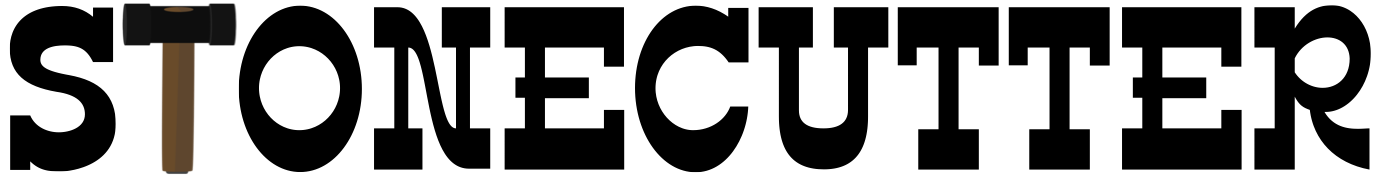
\includegraphics[width=5in]{figures/stonecutter.png} % Include the logo
\end{center}
\end{figure}
%-- end TCL logo

\maketitle % Insert the title, author and date
\thispagestyle{fancy} %-- force the fancyhdr

\begin{center}
\begin{tabular}{l r}
Date: & January 22, 2019 \\ % Date the experiment was performed
Revision: & 0.1 \\         % revision number
Authors: & Tactical Computing Labs\\ % Author names
& contact@tactcomplabs.com\\
\end{tabular}
\end{center}

% If you wish to include an abstract, uncomment the lines below
% \begin{abstract}
% Abstract text
% \end{abstract}

%----------------------------------------------------------------------------------------
%       TOC
%----------------------------------------------------------------------------------------

\clearpage
\tableofcontents
\clearpage

%----------------------------------------------------------------------------------------
%       List of Document Elements
%----------------------------------------------------------------------------------------

\clearpage
\listoffigures
\lstlistoflistings
\listoftables
%\listofalgorithms
\clearpage

%----------------------------------------------------------------------------------------
%       Changelog
%----------------------------------------------------------------------------------------

\clearpage
\begin{versionhistory}
  \vhEntry{0.1}{01.22.2018}{JLeidel}{Initial public release}
\end{versionhistory}

\clearpage

%----------------------------------------------------------------------------------------
%	SECTION 1
%----------------------------------------------------------------------------------------
\clearpage
\section{Overview}

this is a citation~\cite{IRSpec}.


The CoreGen Intermediate Representation (IR) specification is utilized as the core 
mechanism by which to translate a hardware design to various levels of hardware 
design language and simulation infrastructure.  The CoreGen IR has the following goals:

\begin{itemize}
\item \textbf{Support Rapid Design Workflows}: Traditional design techniques and tools require long 
design and prototyping cycles, often with expensive external tools.  The CoreGen IR is design to provide 
rapid design and prototyping workflows such that hardware and software artifacts can be generated in minutes 
rather than days.

\item \textbf{Preserve Hardware Dependencies}: The CoreGen IR is designed to preserve the dependency 
between individual hardware modules and their constituent submodules.  These dependencies are preserved 
in a manner similar to traditional compiler technology, e.g. a \textit{directed acyclic graph} (DAG).  These 
dependencies are subsequently utilized to analyze certain inherent properties of the DAG in order to 
verify, optimized and document the design.  

\item \textbf{Support Modular Design Principles/Reuse}: One of the principle issues that plague previous 
design workflows and paradigms is the lack of potential reuse.  The CoreGen IR provides modular reuse 
of individual design elements as well as the ability to use design templates to rapidly build similar, but 
specialized design elements.  Further, all individual hardware modules can be overridden using external 
design elements in order to further construct specialized designs.  

\item \textbf{Support High-Level Design Verification}: One of the primary goals of the CoreGen infrastructure 
is the ability to perform high performance, low latency design verification without the need to perform low-level 
synthesis and simulation.  This capability is provided by the inherent ability to express complex designs 
within the CoreGen IR.  

\item \textbf{Support Multiple Artifact Generation}: The final goal of the CoreGen IR is to drive secondary 
and, potentially, external tooling.  These tools provide the ability to generate multiple levels of hardware 
design language for the complementary architecture as well as the potential to generate software 
artifacts such as compiler tool chains from the design description.
\end{itemize}

The CoreGen IR is constructed using the standard \textit{YAML}~\cite{YAML} format.  This is a human 
readable text structure that preserves both descriptions of individual hardware modules and 
references between adjacent modules (the DAG from above).  YAML is formatted using blocks of 
\textit{Collections}.  Collections describe an individual type of node (hardware module) in the CoreGen 
IR.  For example, the notion of a register file is encapsulated in a single collection.  Each collection 
may contain a set of \textit{sequences}.  These sequences are individual instances of the appropriate 
module type are denoted with a name followed by a colon (NAME:).  
For example, your design may include multiple different register files, each represented 
as a sequence.  Each sequence will include some number of elements, each denoted with a name followed 
by a dash (NAME-).  These sequence instances may also include a hierarchical set of sequences with scalar 
values.  The named elements and their associated scalar values are marked using the name and colon designator (NAME:).  
These sub-sequences and associated scalars represent the various design parameters for the 
target instance of the target node type.  In our example, a register file may contain some number of registers.  
Each register has a name, index value, bit width and other such parameters.  Each specific node type includes 
unique, recognizable scalar parameters (detailed in the sections below).  The scalar values assigned to each parameter 
may include text, boolean values (\texttt{true}, \texttt{false}), integers and floating point values.  

The YAML formatting paradigm uses indentation (spaces, \textit{NOT} tabs) in order to define hierarchies 
and inheritance.  For example, in our register node description, you'll find that there is a top-level \texttt{Register} 
designator with multiple sequences of registers, each marked with a top-level \texttt{RegName} to denote 
an individual register.  We see an example of this in Listing~\ref{lis:sampleindent}.  

Given the textual nature of the CoreGen intermediate representation, there are no external 
packages required to read and/or write the IR.  However, we \textit{highly} recommend that 
you utilize the integrated CoreGen tooling in order to maintain the internal dependencies and 
verify the syntactical correctness of the IR.  Further, parsing the YAML using non-CoreGen 
tools may result in unresolved internal dependency links due to incorrect parsing order.  
Regardless of the format of the IR text, the CoreGen tools will parse the file in the correct nodal 
order.  

 
%----------------------------------------------------------------------------------------
%	SECTION 2
%----------------------------------------------------------------------------------------
\clearpage
\section{StoneCutter Language}
\label{sec:StoneCutterLanguage}


\subsection{Overview}
\label{sec:LangOverview}

\subsection{Register Class Definitions}
\label{sec:RegClassDef}

\subsection{Instruction Prototypes}
\label{sec:InstructionPrototypes}

\subsection{Variable Definitions}
\label{sec:Variable Definitions}

\subsection{Arithmetic Operations}
\label{sec:Arithmetic Operations}

\subsection{Conditional Operations}
\label{sec:ConditionalOperations}

\subsection{Loop Operations}
\label{sec:LoopOperations}

%----------------------------------------------------------------------------------------
%	SECTION 3
%----------------------------------------------------------------------------------------
\clearpage
\section{Intrinsic Functions}
\label{sec:IntrinsicFunctions}

\subsection{Overview}
\label{sec:IntrinsicOverview}

\subsection{Arithmetic Intrinsics}
\label{sec:ArithIntrinsics}

\subsubsection{CLZ}
\label{sec:CLZ}

\subsubsection{COMPRESS}
\label{sec:COMPRESS}

\subsubsection{COMPRESSM}
\label{sec:COMPRESSM}

\subsubsection{CTZ}
\label{sec:CTZ}

\subsubsection{DOZ}
\label{sec:DOZ}

\subsubsection{EXTRACTS}
\label{sec:EXTRACTS}

\subsubsection{EXTRACTZ}
\label{sec:EXTRACTZ}

\subsubsection{INSERTS}
\label{sec:INSERTS}

\subsubsection{INSERTZ}
\label{sec:INSERTZ}

\subsubsection{MAJ}
\label{sec:MAJ}

\subsubsection{MAX}
\label{sec:MAX}

\subsubsection{MERGE}
\label{sec:MERGE}

\subsubsection{MIN}
\label{sec:MIN}

\subsubsection{NOT}
\label{sec:NOT}

\subsubsection{POPCOUNT}
\label{sec:POPCOUNT}

\subsubsection{REVERSE}
\label{sec:REVERSE}

\subsubsection{ROTL}
\label{sec:ROTL}

\subsubsection{ROTR}
\label{sec:ROTR}

\subsubsection{SEXT}
\label{sec:SEXT}

\subsubsection{ZEXT}
\label{sec:ZEXT}

\clearpage
\subsection{Memory Intrinsics}
\label{sec:MemIntrinsics}

\subsubsection{LOAD}
\label{sec:LOAD}

\subsubsection{STORE}
\label{sec:STORE}




%----------------------------------------------------------------------------------------
%	SECTION: Appendix A: Sample IR
%----------------------------------------------------------------------------------------
\clearpage
\section{Appendix A: Sample StoneCutter Implementation}
\label{sec:AppendixA}

\vspace{0.125in}
\lstinputlisting[frame=single,style=base,caption={Sample StoneCutter},captionpos=b,label={lis:samplescfile}]{SAMPLE.sc}

%----------------------------------------------------------------------------------------
%	SECTION: Appendix B: Intrinsic Operation Table
%----------------------------------------------------------------------------------------
\clearpage
\section{Appendix B: Intrinsic Function Table}
\label{sec:AppendixB}

%----------------------------------------------------------------------------------------
%	BIBLIOGRAPHY
%----------------------------------------------------------------------------------------

\clearpage
\bibliography{refs.bib}
\bibliographystyle{IEEEtran}


%----------------------------------------------------------------------------------------


\end{document}
